%!TEX root = ../../super_main.tex
\chapter{Introduction}
\label{cha:introduction}

\todo[inline]{Insert mild intro. Techonology helps our lives get better -> Folk with autism can be helped}

% Purpose of software
This report focuses on the continued development of an existing \emph{Android}-software suite for tablets called \giraf(Graphical Interface Resources for Autistic Folk), which includes tools and games to assist and train everyday aspects of life for citizens diagnosed an Autism Spectrum Disorder (ASD) and their guardians. 

One motivation for this tool is to digitize some of the existing tools that people with an autism disorder, already uses. 

One of the main stakeholder of the \giraf-system is a kindergarten called \emph{Birken} for children diagnosed with an ASD. In this kindergarten the staff spends a lot of time preparing visual schedules and checklists for the children which helps with their daily functions. 
 %for them to be better to understand basic social strategies. 
This could be for instance be a schedule for the day for a child, constructed of pictograms, simple pictures, laminated and applied to different surfaces using Velcro-tape for the children to inspect.

\begin{table}[!htbp]
    \begin{tabular}{|l|l|l|}
    \hline
    \textbf{Role}				& \textbf{Group}  & \textbf{Description}                                   \\ \hline
    \multirow{2}{*}{Users}      & Citizen         & Citizens diagnosed with ASD                            \\ \cline{2-3}
             					& Guardian        & Institutional guardians of citizens diagnosed with ASD \\ \hline
    Costumers 					& Social services & The municipality of Aalborg                            \\ \hline
    \end{tabular}
\end{table}
\todo[inline]{Refer to this table and add caption and label OR just describe this in text}

%!TEX root = ../../super_main.tex

\section{Multi project organization}

This semester project is the continuation of a widely spanning multi project with 52 developers which are organized in 14 smaller groups, up to four developers per group, including a group consisting of the authors of this report. The multi project was split into 3 different project areas: Build and Deployment, GUI, Database. 

\subsection{Organization}
The multi project was organized using the development method Scrum\parencite{scrum}, more specific Scrum of Scrums. This method alows the multiproject to be self-organized and enforces the individual groups to do work more independetly. This independent work fits great in since the individual groups is used to work in smaller projects groups. However in this semetester the groups will now obtain experience in working on a larger scale projects than previous encountered in their education. 
\\\\
As seen in \figref{fig:scrum_of_scrums} the Scrum of Scrums is split into three levels. The bottom most level is the individual groups, which work exactly as an ordinary development group using the Scrum method. The middle layer contains the three project areas where representatives from each individual group meet and syncronize their work at least twice a week. The top layer in \figref{fig:scrum_of_scrums} contains representatives from all of the project areas. However since standup meeting only occur once a week in this Scrum representatives from all groups are encouraged to join the meetings.

\todo[inline]{Update Figure}
\begin{figure}[!htbp]
  \centering
    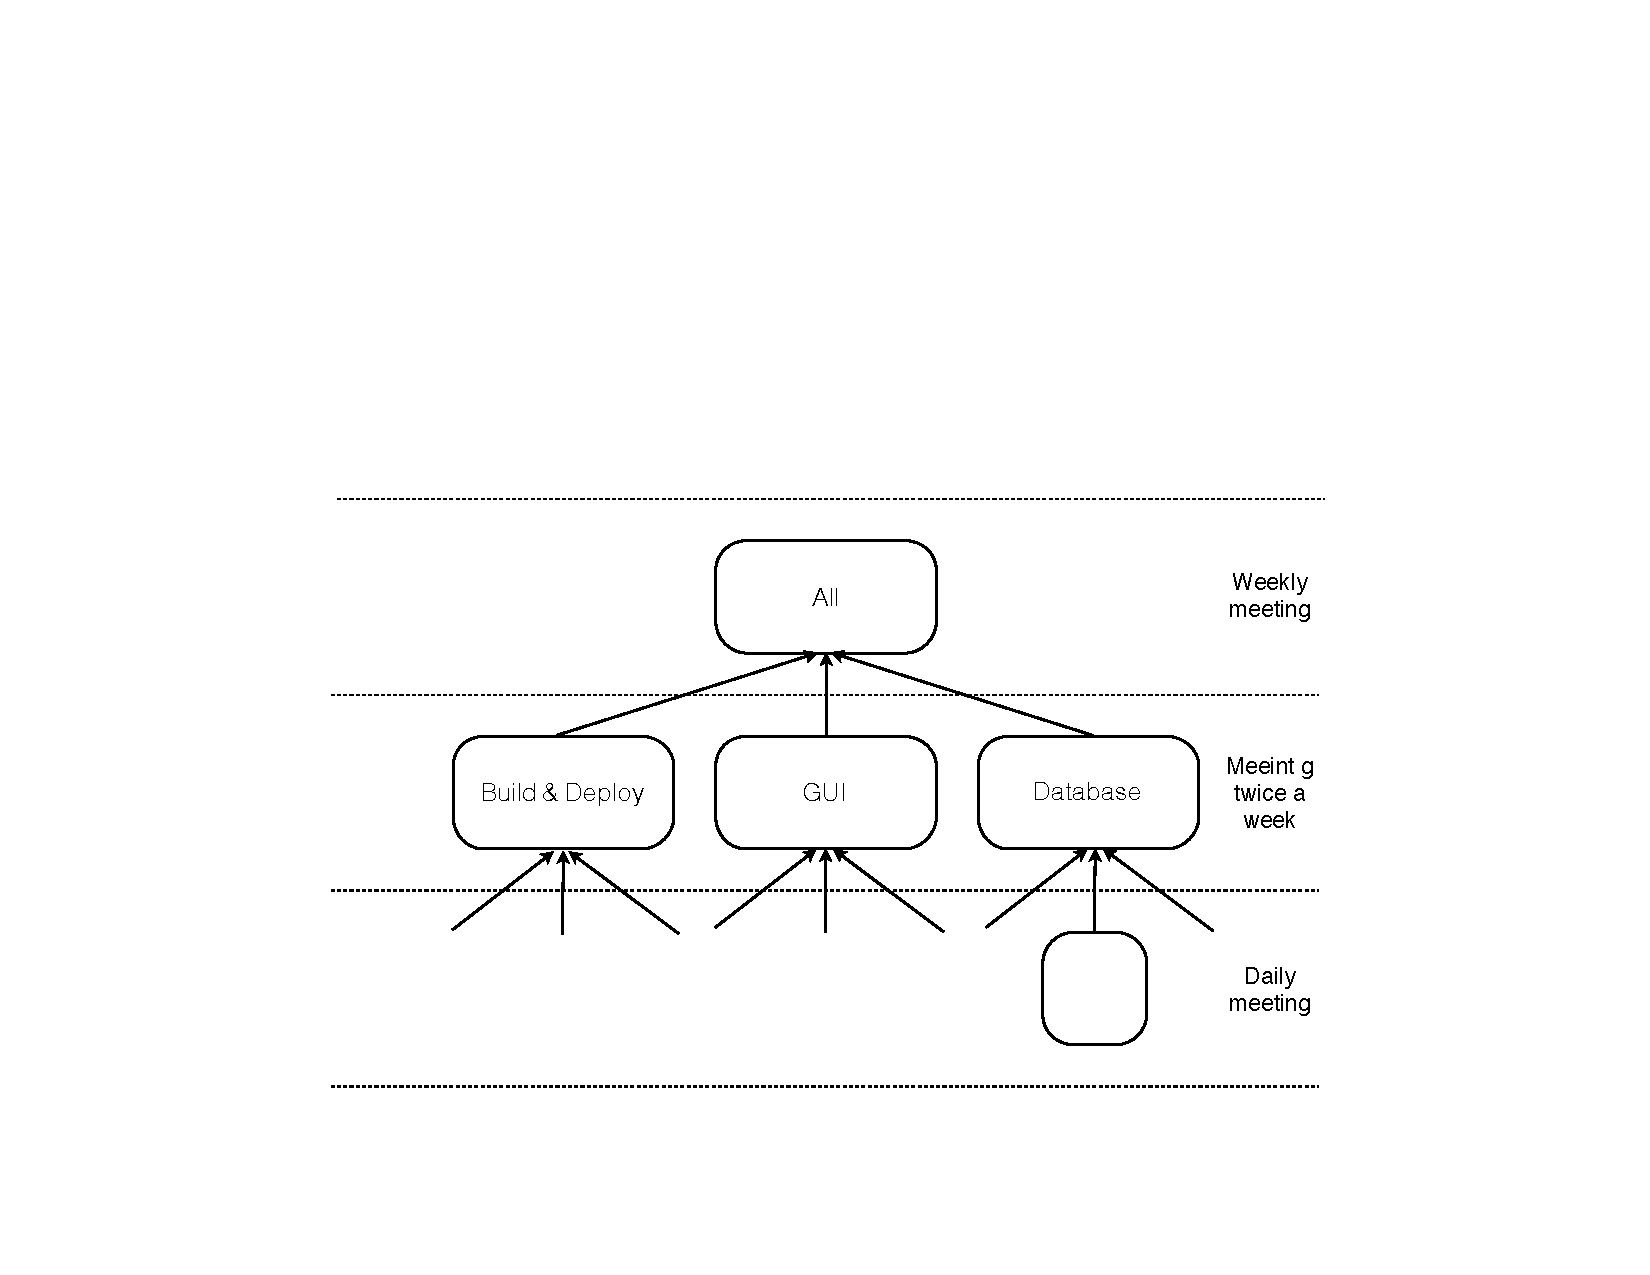
\includegraphics[width=0.6\textwidth]{scrum_of_scrums}
    \caption{Organization in Scrum of Scrums.}
    \label{fig:scrum_of_scrums}
\end{figure}



\subsection{Roles and Responsibilities}
Several different roles and responsibilities were divided among the project groups. This group volunteered as ``Webadmin'' and also included an Android Guru.

The ``Webadmin'' responsibility included administration of the official \giraf web page. 

